% !TeX root = ./2021-22-COMP250-01-session-materials_screen.tex

% Adjust these for the path of the theme and its graphics, relative to this file
%\usepackage{beamerthemeFalmouthGamesAcademy}
\usepackage{../../beamerthemeFalmouthGamesAcademy}
\usepackage{multimedia}
\graphicspath{ {../../} }

% Default language for code listings
\lstset{language=C++,
        morekeywords={each,in,nullptr}
}

% For strikethrough effect
\usepackage[normalem]{ulem}
\usepackage{wasysym}

% https://tex.stackexchange.com/a/42620
\usepackage{pifont}% http://ctan.org/pkg/pifont
\newcommand{\cmark}{\ding{51}}%
\newcommand{\xmark}{\ding{55}}%

\usepackage{algpseudocode}

\usepackage{pdfpages}

% http://www.texample.net/tikz/examples/state-machine/
\usetikzlibrary{arrows,automata}

\newcommand{\modulecode}{COMP260}\newcommand{\moduletitle}{Distributed Systems}\newcommand{\sessionnumber}{5}

\begin{document}
\title{\sessionnumber: Introduction to AI}
\subtitle{\modulecode: \moduletitle}

\frame{\titlepage} 

\begin{frame}{Proposal}
        \begin{itemize}
                \pause\item For next week!
                \pause\item Prepare a 1-2 page proposal document covering the following:
                \begin{itemize}
                        \pause\item What is the high concept of your computing artefact?
                        \pause\item What functionality will your component include?
                        \pause\item How does your component fit into your chosen specialism?
                        \pause\item Why is this artefact needed?
                        \pause\item What are the key requirements?
                        \pause\item Is the scope appropriate for the product development time-frame?
                        \pause\item How will you address the architect and research requirement?
                \end{itemize}
        \end{itemize}
\end{frame}

\part{What is AI?}
\frame{\partpage}

\begin{frame}{What is AI?}
	\begin{itemize}
		\item Socrative FALCOMPED
		\item Discuss for \textbf{5 minutes}
		\item Suggest a \textbf{one sentence} definition of artificial intelligence (AI)
	\end{itemize}
\end{frame}

\iftoggle{printable}{
	% Skip this slide
}{
	\begin{frame}{What is AI?}
		\begin{itemize}
			\pause\item An AI is a \textbf{machine} (or piece of \textbf{software})
				which performs tasks requiring \textbf{intelligence}
			\pause\item Intelligence is making \textbf{decisions} to achieve \textbf{goals} --- roughly, what brains do
		\end{itemize}
	\end{frame}
}

\begin{frame}{What isn't AI?}
	\begin{itemize}
		\pause\item AI implies something beyond ``mere computation'' --- but the lines are sometimes blurry
		\pause\item AI is \textbf{not necessarily} about:
			\begin{itemize}
				\pause\item Mimicking human intelligence
				\pause\item General intelligence
				\pause\item Learning
			\end{itemize}
		\pause\item ... although these are all important sub-fields of AI
	\end{itemize}
\end{frame}

\begin{frame}{Computers vs brains}
	Discuss:
	\begin{itemize}
		\pause\item For what kinds of tasks are digital computers ``better'' than human brains?
		\pause\item For what kinds of tasks are human brains ``better'' than digital computers?
		\pause\item For what kinds of tasks are both ``good'', but approach the task in different ways?
	\end{itemize}
\end{frame}

\begin{frame}{Is it AI?}
	Discuss: are these examples of AI?
	\begin{columns}
		\begin{column}{0.48\textwidth}
			\begin{itemize}
				\pause\item Calculator
				\pause\item Computer opponent in a chess program
				\pause\item Enemy in a video game
				\pause\item Facebook newsfeed
				\pause\item Autocorrect in a text messaging app
				\pause\item Autocompletion in an IDE
				\pause\item Spellchecker
			\end{itemize}
		\end{column}
		\begin{column}{0.48\textwidth}
			\begin{itemize}
				\pause\item Satellite navigation
				\pause\item Virtual assistant (e.g.\ Siri, Alexa, Cortana etc.)
				\pause\item Amazon product recommendations
				\pause\item Search function in a text editor
				\pause\item Google search
				\pause\item C++ compiler
				\pause\item Robot
			\end{itemize}
		\end{column}
	\end{columns}
\end{frame}


%\part{Module Introduction}
\frame{\partpage}

\begin{frame}{Aim}
    \begin{center}
        To research and apply creative computing to the domain of artificial intelligence for games.
    \end{center}
\end{frame}

\begin{frame}{Description}
    On this module, you learn how to apply artificial intelligence in the context of games. You will gain in understanding and experience of the technical dimension of artificial intelligence and you could leverage it in the particular expressive context within game development. You will apply your learning in a practical context where you will design artificially intelligent agents for a game in a live brief format, taking as your cue the game’s concept.
\end{frame}

\begin{frame}{Learning Outcomes}
    \begin{itemize}
        \item \textbf{2: Architect}. Integrate appropriate data structures and interoperating components into software, with reference to their merits and flaws.
        \item \textbf{5: Research}. Develop an argument on a topic using appropriate research methods, primary and secondary sources, and academic conventions.
    \end{itemize}
\end{frame}

\begin{frame}{Roadmap}
    \begin{itemize}
        \pause\item Weekly \textbf{lectures} with me
        \pause\item Weekly \textbf{portfolio development workshops} with Kate Bergel (joint with COMP210, COMP220, COMP260)
        \pause\item Fortnightly \textbf{supervisions} (project check-ins) with me
        \pause\item Timetable towards end of study block is currently undergoing changes --- as always, check MyTimetable regularly for updates
        \pause\item Check MyFalmouth for assignment deadlines
    \end{itemize}
\end{frame}

%\part{Assignments}
\frame{\partpage}

\begin{frame}{COMP250 assignments}
	\pause Similar to COMP220:
	\begin{itemize}
		\pause\item Portfolio task (90\%)
		\pause\item Research journal (10\%)
	\end{itemize}
\end{frame}

\begin{frame}{COMP250 portfolio task}
	\begin{itemize}
		\pause\item Assignment brief on LearningSpace
		\pause\item Basically, develop an \textbf{AI component} for a game
		\pause\item In the next two weeks:
			\begin{itemize}
				\pause\item Prepare a \textbf{proposal}
				\pause\item Start \textbf{collecting} and \textbf{reading} appropriate literature
			\end{itemize}
		\pause\item For the rest of today: begin preparing your \textbf{proposal}
		\pause\item Not sure what's technically feasible? \textbf{Ask me!}
	\end{itemize}
\end{frame}


\newcommand{\pictureslideb}[3]{
	\begin{frame}{#1}
		\begin{center}
			#3
			
			\vspace{6pt}
			
			\includegraphics[height=0.6\textheight]{#2}
		\end{center}
	\end{frame}
}

\newcommand{\pictureslide}[2]{
	\begin{frame}{#1}
		\begin{center}
			\includegraphics[height=0.6\textheight]{#2}
		\end{center}
	\end{frame}
}

\part{AI in games}
\frame{\partpage}

\begin{frame}{Applications of AI in games}
	\begin{itemize}
		\pause\item Enemies and other NPCs
		\pause\item Opponents in $\{$board, card, strategy$\}$ games
		\pause\item Automated playtesting
		\pause\item Directors, hints, adaptive difficulty
		\pause\item Procedural content generation
		\pause\item Content production tools
		\pause\item Procedural narrative
		\pause\item Agent-based simulations
		\pause\item ...
	\end{itemize}
\end{frame}

\begin{frame}{Why game AI?}
	\begin{itemize}
		\pause\item Games are a useful testbed for new AI technologies
		\pause\item Game theory is a useful mathematical abstraction for many types of problem
		\pause\item Game AI is more than pure problem solving --- game AI needs to create an entertaining experience
	\end{itemize}
\end{frame}

\pictureslide{Nimrod (Ferranti, 1951)}{nimrod}
\pictureslide{Samuel's Checkers program (IBM, 1962)}{samuel}
\pictureslide{Galaxian (Namco, 1979)}{galaxian}
\pictureslide{Pac-Man (Namco, 1980)}{pacman}
\pictureslide{Deep Blue (IBM, 1997)}{deep_blue}
\pictureslide{Half-Life (Valve, 1998)}{half_life}
\pictureslide{The Sims (Maxis, 2000)}{sims}
\pictureslide{Black \& White (Lionhead, 2001)}{black_white}
\pictureslide{Halo 2 (Bungie, 2004)}{halo2}
\pictureslide{F.E.A.R. (Monolith Productions, 2005)}{fear}
\pictureslide{Fa\c{c}ade (Mateas \& Stern, 2005)}{facade}
\pictureslide{Chinook (Schaeffer et al, 2007)}{chinook}
\pictureslide{Left 4 Dead (Valve, 2008)}{left_4_dead}
\pictureslide{Watson (IBM, 2011)}{watson}
\pictureslide{Deep learning for Atari games (DeepMind, 2013)}{deepmind_atari}
\pictureslide{AlphaGo (Google DeepMind, 2016)}{alphago}
\pictureslide{AlphaStar (Google DeepMind, 2019)}{alphastar}

% \begin{frame}{What will we be covering?}
% 	\begin{itemize}
% 		\pause\item Finite state machines
% 		\pause\item Behaviour trees
% 		\pause\item Game theory
% 		\pause\item Planning
% 		\pause\item Utility-based AI
% 		\pause\item Game tree search
% 		\pause\item Procedural content generation
% 		\pause\item Multi-agent systems
% 		\pause\item Pathfinding and navigation
% 		\pause\item Evolutionary algorithms
% 		\pause\item Artificial neural networks
% 	\end{itemize}
% \end{frame}

\part{AI architectures}
\frame{\partpage}

\begin{frame}{Rule-based AI}
	Generally implemented as \texttt{if} statements or event-based triggers
\end{frame}

\begin{frame}{Finite state machines}
	\begin{center}
		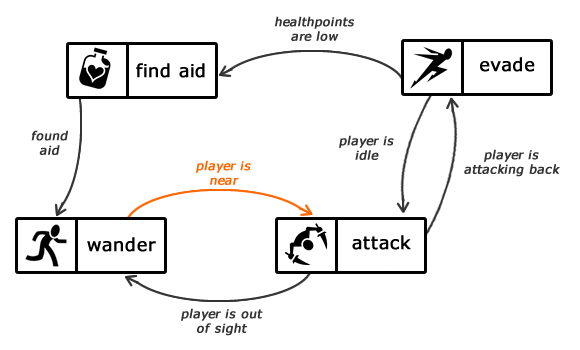
\includegraphics[width=\textwidth]{fsm_enemy_brain}
		% https://gamedevelopment.tutsplus.com/tutorials/finite-state-machines-theory-and-implementation--gamedev-11867
	\end{center}
\end{frame}

\begin{frame}{Behaviour trees}
	\begin{center}
		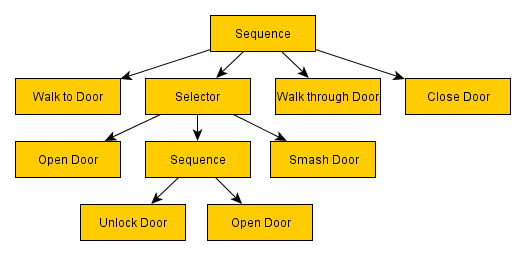
\includegraphics[width=\textwidth]{behaviour_tree}
		% https://www.gamasutra.com/blogs/ChrisSimpson/20140717/221339/Behavior_trees_for_AI_How_they_work.php
	\end{center}
\end{frame}

\begin{frame}{Game tree search}
	\begin{center}
		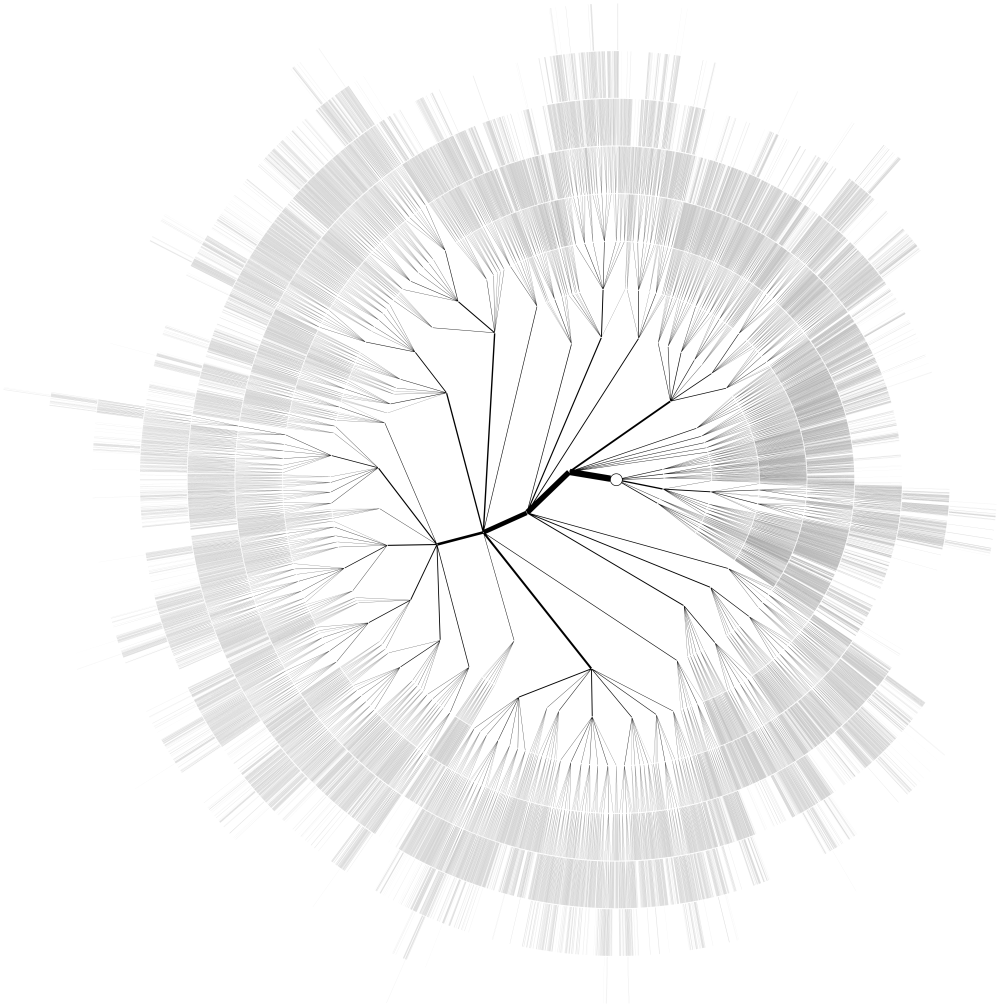
\includegraphics[height=0.7\textheight]{mcts}
	\end{center}
\end{frame}

\begin{frame}{Multi-agent approaches (e.g.\ flocking)}
	\begin{center}
		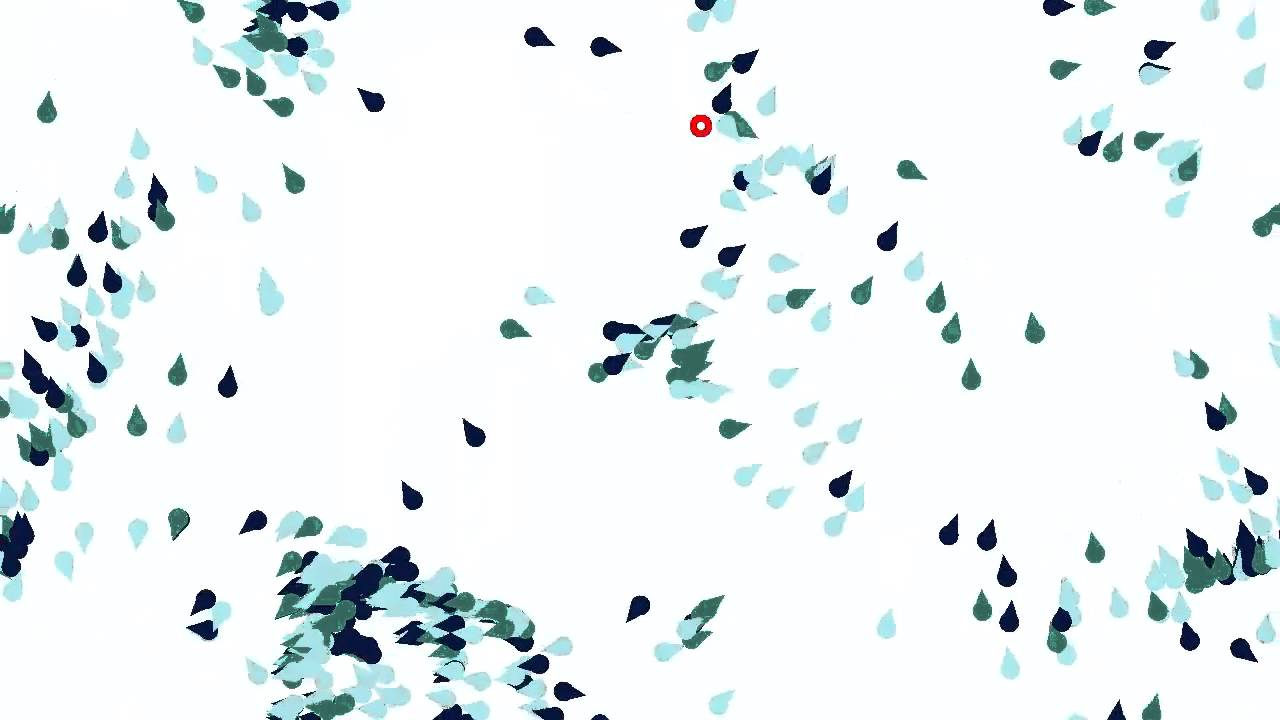
\includegraphics[width=\textwidth]{flocking}
		% https://www.youtube.com/watch?v=5p6OAEVKw-0
	\end{center}
\end{frame}

\begin{frame}{Machine learning}
	\begin{center}
		\colorbox{white}{
			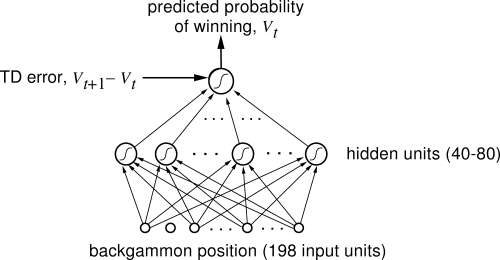
\includegraphics[width=0.7\textwidth]{tdgammon}
		}
		% https://users.auth.gr/kehagiat/Research/GameTheory/12CombBiblio/BackGammon.html
	\end{center}
\end{frame}

\begin{frame}{AI architectures}
	\begin{itemize}
		\pause\item Can roughly be divided into \textbf{hand-authored}...
			\begin{itemize}
				\pause\item Rule-based, FSM, behaviour trees
			\end{itemize}
		\pause\item ... and \textbf{computational intelligence}
			\begin{itemize}
				\pause\item Search, multi-agent, machine learning
			\end{itemize}
		\pause\item Do you want to \textbf{design} the AI behaviours yourself,
			or do you want them to \textbf{emerge} from the system?
		\pause\item Predictability and authorial control versus adaptability and novelty
		\pause\item Can also combine the two
			\begin{itemize}
				\pause\item E.g.\ use a rule-based system to constrain a CI system
				\pause\item E.g.\ flocking --- individual agents are usually rule-based, but overall flock dynamics
					are emergent
			\end{itemize}
	\end{itemize}
\end{frame}


\begin{frame}{Workshop}
        \begin{itemize}
                \item Begin (or continue) preparing your \textbf{proposal}
                \item Discuss and brainstorm your ideas with your peers
                \item Ask me for feedback or suggestions!
        \end{itemize}
\end{frame}

\end{document}
